En la figura \ref{fig:db} se aprecia el modelo de datos del sistema y se describen las entidades que lo conforman, así como los respectivos atributos de cada una de estas entidades.
\begin{figure}[h]
	\centering
	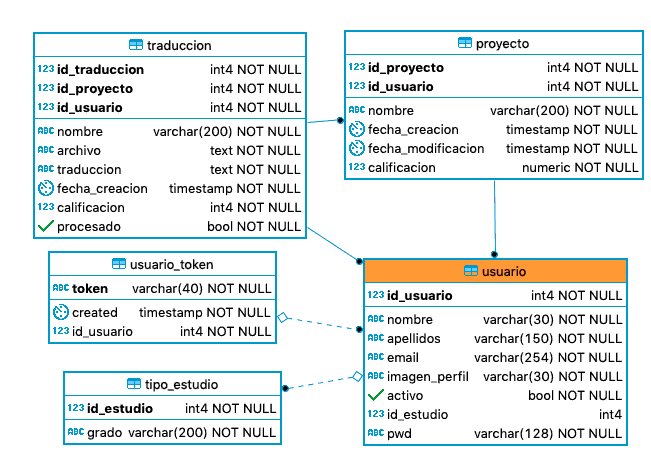
\includegraphics[width=\textwidth]{capitulo4/imagenes/tt_base.png}
	\caption{Modelo de datos del sistema.}
	\label{fig:db}
\end{figure}

\subsection{Entidad: Usuario}
Se refiere a la cuenta que un usuario puede tener, es la forma en la que accede al sistema.
\subsubsection{Atributos}
\begin{center}
	\begin{longtable}{|J{3cm}|J{4cm}|J{3cm}|J{2cm}|J{2cm}|}
		\hline
		\textbf{Nombre} & \textbf{Descripción} & \textbf{Tipo} & \textbf{Requerido} & \textbf{Único} \\ \hline
		id & Llave primaria autoincrementable del usuario & integer & Sí & Sí\\ \hline
		nombre & Nombre que tiene un usuario & varchar(30) & Sí & No \\ \hline
		apellidos & Apellidos de un usuario & varchar(150) & Sí & No \\ \hline
		email & Correo electrónico asociado a un usuario & varchar(254) & Sí & Sí\\ \hline
		imagen\_perfil & Ruta relativa de la ubicación de la imagen de perfil del usuario & varchar(30) & Sí & No \\ \hline
		activo & Bandera que nos permite saber si un usuario ha verificado su cuenta & boolean & Sí & No \\ \hline
		id\_estudios & Identificador para relacionar al usuario con el grado de estudio que tiene del catalogo de tipos de estudios & integer & No & No \\ \hline
		password & Contraseña cifrada del usuario & varchar(128) & Sí & No \\ \hline
		\caption{Tabla de los atributos de la entidad usuario}
		\label{tbl:entidad-usuario}
	\end{longtable}
\end{center}
\subsection{Entidad: Proyecto}
Se refiere a los proyectos que están asociados a un usuario, un proyecto esta compuesto por varias traducciones.
\subsubsection{Atributos}
\begin{center}
	\begin{longtable}{|J{3cm}|J{4cm}|J{3cm}|J{2cm}|J{2cm}|}
		\hline
		\textbf{Nombre} & \textbf{Descripción} & \textbf{Tipo} & \textbf{Requerido} & \textbf{Único} \\ \hline
		id\_proyecto & Identificador autoincrementable del proyecto, forma parte de la llave primaria & integer & Sí & Sí \\ \hline
		id\_proyecto & Identificador del usuario que tiene el proyecto, forma parte de la llave primaria & integer & Sí & No \\ \hline
		nombre & Nombre del proyecto & varchar(200) & Sí & No \\ \hline
		fecha\_modificacion & Fecha que se actualiza cada vez que se modifica el proyecto & timestamp & Sí & No \\ \hline
		fecha\_creacion & Fecha en la cual se crea el proyecto & timestamp & Sí & No \\ \hline
		calificacion & Calificación que se calcula a través de las calificaciones de las traducciones asociadas con el proyecto, puede contener decimales & numeric & Sí & No \\ \hline
		\caption{Tabla de los atributos de la entidad proyecto}
		\label{tbl:entidad-proyecto}
	\end{longtable}
\end{center}
\subsection{Entidad: Traducción}
Hace referencia a la traducción de \LaTeX que forma parte de un proyecto y que pertenece a un usuario. Esta traducción es el resultado de analizar una imagen.
\subsubsection{Atributos}
\begin{center}
	\begin{longtable}{|J{3cm}|J{4cm}|J{3cm}|J{2cm}|J{2cm}|}
		\hline
		\textbf{Nombre} & \textbf{Descripción} & \textbf{Tipo} & \textbf{Requerido} & \textbf{Único} \\ \hline
		id\_traduccion & Identificador autoincrementable de la traducción, forma parte de la llave primaria & integer & Sí & Sí \\ \hline
		id\_proyecto & Identificador del proyecto al cual pertenece la traducción, forma parte de la llave primaria & integer & Sí & No \\ \hline
		id\_usuario & Identificador del usuario, forma parte de la llave primaria & integer & Sí & No \\ \hline
		nombre & Nombre que se le da a la traducción & varchar(200) & Sí & No \\ \hline
		traduccion & Traducción generada & text & Sí & No \\ \hline
		archivo & Ruta de la imagen a traducir & text & Sí & No \\ \hline
		calificacion & Calificación que se le da a la traducción para retroalimentación del usuario y del sistema & integer & Sí & No\\ \hline
		fecha\_creacion & Fecha en la cual se crea la traducción & timestamp & Sí & No \\ \hline
		procesado & Indica si la imagen ya asociada a la traducción ya ha sido procesada & boolean & Sí & No\\ \hline
		\caption{Tabla de los atributos de la entidad traducción}
		\label{tbl:entidad-traduccion}
	\end{longtable}
\end{center}
\subsection{Entidad: Tipo estudios}
Hace referencia a los distintos grados de estudios que tiene un usuario.
\subsubsection{Atributos}
\begin{center}
	\begin{longtable}{|J{3cm}|J{4cm}|J{3cm}|J{2cm}|J{2cm}|}
		\hline
		\textbf{Nombre} & \textbf{Descripción} & \textbf{Tipo} & \textbf{Requerido} & \textbf{Único} \\ \hline
		id & Llave primaria autoincrementable & integer & Sí & Sí \\ \hline
		grado & Nombre del grado de estudio & varchar(200) & Sí & No \\ \hline
		\caption{Tabla de los atributos de la entidad tipo de estudios}
		\label{tbl:entidad-tipo-estudios}
	\end{longtable}
\end{center}
\subsection{Entidad: Usuario Token}
Se refiere al token de autenticación que tiene un usuario al momento de crear una cuenta y que su utiliza en la comunicación entre la aplicación web y android.
\subsubsection{Atributos}
\begin{center}
	\begin{longtable}{|J{3cm}|J{4cm}|J{3cm}|J{2cm}|J{2cm}|}
		\hline
		\textbf{Nombre} & \textbf{Descripción} & \textbf{Tipo} & \textbf{Requerido} & \textbf{Único} \\ \hline
		token & Llave primaria y token de autenticación del usuario para la API REST & varchar(40) & Sí &  Sí\\ \hline
		created & Fecha de generación del token & timestamp & Sí & No\\ \hline
		id\_usuario & Identificador del usuario al que pertenece el token& integer & Sí & No\\ \hline
		\caption{Tabla de los atributos de la entidad usuario token}
		\label{tbl:entidad-usuario-token}
	\end{longtable}
\end{center}